% !TEX program = pdflatex
\documentclass[aspectratio=169,10pt]{beamer}

\usetheme[progressbar=frametitle]{metropolis}
\setbeamertemplate{frame numbering}[fraction]
\metroset{block=fill}

\usepackage[utf8]{inputenc}
\usepackage[T1]{fontenc}
\usepackage{microtype}
\usepackage{amsmath, amssymb, amsthm}
\usepackage{booktabs}
\usepackage{tikz}
\usetikzlibrary{positioning,fit,backgrounds,arrows.meta}
\usepackage{xcolor}

% Convenience macros that match the paper.
\newcommand{\rfmm}[3]{\omega(#1,#2,#3)}
\newcommand{\bigO}{O}

% Title-page data.
\title{Counting 4-Cycles in Fully Dynamic Graphs}
\subtitle{A Cyclic-Join Perspective}
\author{Speaker 1 \and Speaker 2 \and Speaker 3 \and Speaker 4}
\institute{Algorithms seminar -- mock PODS 2025}
\date{}

\begin{document}

% ---------------------------------------------------------------
\begin{frame}[plain]
  \titlepage
\end{frame}

% =========================================================================
% Speaker 1 -- The problem (3:30)
% =========================================================================

% ---------------------------------------------------------------
\begin{frame}{The problem, in one picture}
  \begin{columns}[T,onlytextwidth]
    \begin{column}{0.55\textwidth}
      \centering
      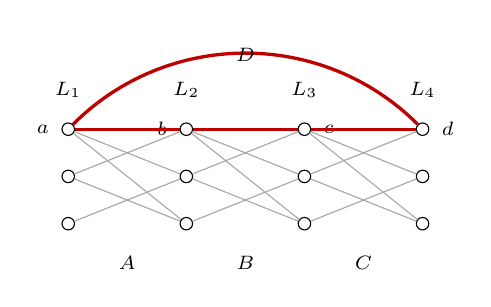
\begin{tikzpicture}[
          every node/.style={font=\scriptsize},
          vert/.style={circle,draw,inner sep=1.2pt,minimum size=4.5pt,fill=white},
          ledge/.style={gray!70,thin},
          hedge/.style={red!75!black,very thick},
        ]
        \foreach \i/\lab in {1/$L_1$,2/$L_2$,3/$L_3$,4/$L_4$} {
          \node at ({(\i-1)*1.5}, 2.1) {\lab};
        }
        \foreach \i in {1,2,3,4} {
          \pgfmathsetmacro{\xx}{(\i-1)*1.5}
          \node[vert] (\i a) at (\xx, 1.6) {};
          \node[vert] (\i b) at (\xx, 1.0) {};
          \node[vert] (\i c) at (\xx, 0.4) {};
        }
        \node[left=1pt of 1a] {$a$};
        \node[left=1pt of 2a] {$b$};
        \node[right=1pt of 3a] {$c$};
        \node[right=1pt of 4a] {$d$};
        \foreach \i/\j in {1/2,2/3,3/4} {
          \draw[ledge] (\i a) -- (\j b);
          \draw[ledge] (\i b) -- (\j a);
          \draw[ledge] (\i b) -- (\j c);
          \draw[ledge] (\i c) -- (\j b);
          \draw[ledge] (\i a) -- (\j c);
        }
        \draw[hedge] (1a) -- (2a);
        \draw[hedge] (2a) -- (3a);
        \draw[hedge] (3a) -- (4a);
        \draw[hedge] (4a) to[bend right=45] (1a);
        \node[font=\scriptsize\itshape] at (0.75, -0.1) {$A$};
        \node[font=\scriptsize\itshape] at (2.25, -0.1) {$B$};
        \node[font=\scriptsize\itshape] at (3.75, -0.1) {$C$};
        \node[font=\scriptsize\itshape] at (2.25, 2.55) {$D$};
      \end{tikzpicture}
    \end{column}
    \begin{column}{0.45\textwidth}
      A four-way \alert{cyclic join} on a database:
      \[
        J \;=\; A \bowtie B \bowtie C \bowtie D
      \]
      \medskip

      Each binary relation is a bipartite edge set between two attribute domains.
      \medskip

      \alert{One tuple in $J$ \;=\; one 4-cycle in the layered graph.}
      \medskip

      So $|J|$ is a count of 4-cycles.
    \end{column}
  \end{columns}
\end{frame}

% ---------------------------------------------------------------
\begin{frame}{What ``fully dynamic'' actually demands}
  Edges arrive and leave one at a time. After every update the system must report the exact 4-cycle count.

  \vspace{0.4em}
  \begin{block}{Cost model: \emph{worst-case} update time}
    The maximum work on \emph{any single} update -- not the average, not the amortised total.
  \end{block}

  \vspace{0.4em}
  Why worst-case, not amortised?
  \begin{itemize}
    \item Databases need \alert{predictable per-update latency}.
    \item A 1-second hiccup once every 1000 updates is a production incident, even if the average is fast.
    \item Stronger guarantee $\Rightarrow$ harder problem.
  \end{itemize}

  \vspace{0.4em}
  The target: beat recompute-from-scratch with a per-update \emph{worst-case} guarantee.
\end{frame}

% =========================================================================
% Speaker 2 -- State of the art & the FMM surprise (3:30)
% =========================================================================

% ---------------------------------------------------------------
\begin{frame}{The landscape: three patterns on $\le 4$ vertices}
  \centering
  \vspace{0.5em}
  \begin{tabular}{lcc}
    \toprule
    Pattern & Best dynamic update time \\
    \midrule
    Triangle (3-cycle) & $\bigO(\sqrt{m})$ \\
    4-clique           & $\bigO(m)$ \\
    \alert{4-cycle}    & \alert{$\bigO(m^{2/3})$} \\
    \bottomrule
  \end{tabular}

  \vspace{1.5em}
  \begin{itemize}
    \item $m$ = number of edges in the host graph.
    \item Two patterns settle at clean exponents; \alert{4-cycles sit at a weird $2/3$}.
    \item That $2/3$ was the state of the art for over a decade.
  \end{itemize}
\end{frame}

% ---------------------------------------------------------------
\begin{frame}{Why is the 4-cycle bound stuck at $m^{2/3}$?}
  Algorithm of Hanauer, Henzinger, Hua (\textit{ICALP 2022}). One-line intuition:

  \vspace{0.4em}
  \begin{itemize}
    \item Split vertices into \alert{low} (degree $\le m^{1/3}$) and \alert{high} (degree $\ge m^{1/3}$).
    \item Maintain a \emph{wedge matrix} $W[u,v]$ \;=\; number of 2-paths $u$--$x$--$v$ with $x$ low-degree.
    \item Each edge update touches at most $m^{1/3} \cdot m^{1/3} = m^{2/3}$ entries of $W$.
  \end{itemize}

  \vspace{0.6em}
  This $m^{1/3}$--$m^{2/3}$ split is the \alert{natural ceiling for combinatorial methods}.

  \vspace{0.4em}
  Matching combinatorial lower bound from OMv conjecture: $\Omega(m^{1/2-\gamma})$ -- doesn't rule out improvement, but the obvious tricks don't help.
\end{frame}

% ---------------------------------------------------------------
\begin{frame}{The 2025 surprise (Assadi \& Shah)}
  \begin{block}{Theorem (Assadi--Shah, PODS 2025)}
    There is an algorithm maintaining the exact 4-cycle count in worst-case time
    \[
      \bigO\!\big(m^{2/3 - \varepsilon}\big), \qquad \varepsilon > 0
    \]
    using \alert{fast matrix multiplication} (FMM).
  \end{block}

  \vspace{0.4em}
  Why is this surprising?
  \begin{itemize}
    \item FMM is a \alert{batch} primitive: multiply two big matrices at once.
    \item Incremental view maintenance is \alert{streaming}: edges arrive one at a time.
    \item Folklore said: \emph{FMM cannot give worst-case dynamic improvements}.
  \end{itemize}

  \vspace{0.4em}
  Their trick: \emph{phases}. Precompute one matrix product across a batch of $m^{1-\delta}$ updates, while answering queries against the \emph{previous} batch.
\end{frame}

% =========================================================================
% Speaker 3 -- Our contribution (3:30)
% =========================================================================

% ---------------------------------------------------------------
\begin{frame}{Re-presenting through a database lens}
  Assadi--Shah is dense. Our lens: \alert{IVM for cyclic joins}.

  \vspace{0.4em}
  \begin{center}
    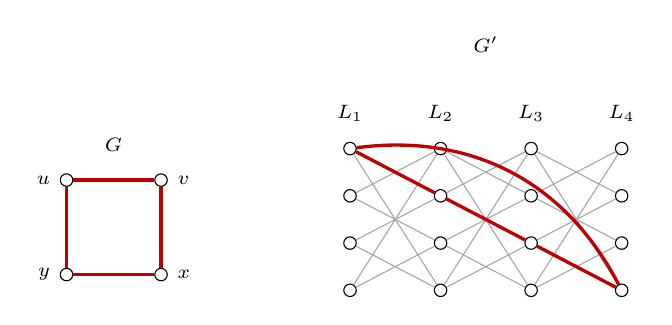
\begin{tikzpicture}[
        every node/.style={font=\scriptsize},
        vert/.style={circle,draw,inner sep=1.2pt,minimum size=4.5pt,fill=white},
        ledge/.style={gray!70,thin},
        hedge/.style={red!75!black,very thick},
      ]
      \begin{scope}[local bounding box=Gbox]
        \node[vert,label=left:$u$]   (gu) at (0.0, 1.2) {};
        \node[vert,label=right:$v$]  (gv) at (1.2, 1.2) {};
        \node[vert,label=right:$x$]  (gx) at (1.2, 0.0) {};
        \node[vert,label=left:$y$]   (gy) at (0.0, 0.0) {};
        \draw[hedge] (gu) -- (gv);
        \draw[hedge] (gv) -- (gx);
        \draw[hedge] (gx) -- (gy);
        \draw[hedge] (gy) -- (gu);
      \end{scope}
      \node[above=2pt of Gbox] {$G$};

      \begin{scope}[xshift=3.6cm,local bounding box=Gpbox]
        \foreach \i/\lab in {1/$L_1$,2/$L_2$,3/$L_3$,4/$L_4$} {
          \node at ({(\i-1)*1.15}, 2.05) {\lab};
        }
        \foreach \i in {1,2,3,4} {
          \pgfmathsetmacro{\xx}{(\i-1)*1.15}
          \node[vert] (u\i) at (\xx, 1.6) {};
          \node[vert] (v\i) at (\xx, 1.0) {};
          \node[vert] (x\i) at (\xx, 0.4) {};
          \node[vert] (y\i) at (\xx,-0.2) {};
        }
        \foreach \i/\j in {1/2,2/3,3/4} {
          \draw[ledge] (u\i) -- (v\j); \draw[ledge] (v\i) -- (u\j);
          \draw[ledge] (v\i) -- (x\j); \draw[ledge] (x\i) -- (v\j);
          \draw[ledge] (x\i) -- (y\j); \draw[ledge] (y\i) -- (x\j);
          \draw[ledge] (y\i) -- (u\j); \draw[ledge] (u\i) -- (y\j);
        }
        \draw[hedge] (u1) -- (v2);
        \draw[hedge] (v2) -- (x3);
        \draw[hedge] (x3) -- (y4);
        \draw[hedge] (y4) to[bend right=35] (u1);
      \end{scope}
      \node[above=12pt of Gpbox] {$G'$};
    \end{tikzpicture}
  \end{center}

  Every general-graph edge $\to$ \alert{4 layered-graph edges}, one per relation. The architecture (degree classes, biadjacency matrices, where each step lives) becomes \emph{visible}.
\end{frame}

% ---------------------------------------------------------------
\begin{frame}{Where the FMM step lives}
  Of the entire machinery, \alert{one product} carries the speedup:
  \[
    A^{L*} \cdot B_{\ell, DD}
    \qquad \text{(rectangular, dimensions $m^{2/3+2\varepsilon} \times m^{1/3-\varepsilon_1+\varepsilon_2}$)}
  \]

  \vspace{0.5em}
  Everything else is bookkeeping:
  \begin{itemize}
    \item degree-class partition (High / Medium / Low; Dense / Sparse),
    \item chunk-based lazy maintenance ($\sqrt{m^{2/3-\varepsilon_1}}$ updates per chunk),
    \item phases for the full general-graph algorithm.
  \end{itemize}

  \vspace{0.4em}
  All of this exists \alert{to feed that one FMM step a well-conditioned input}.

  \vspace{0.4em}
  \emph{This} is the load-bearing line. The constraint system tells us so.
\end{frame}

% ---------------------------------------------------------------
\begin{frame}{Closed-form certificate at \texorpdfstring{$\omega = 2$}{omega = 2}}
  Assadi--Shah's feasibility argument: numerical, at the current $\omega < 2.371339$.

  \vspace{0.4em}
  \alert{Our contribution:} closed-form solution at the conjectural optimum $\omega = 2$.

  \vspace{0.4em}
  \begin{block}{Lemma (Closed-form feasibility at $\omega = 2$)}
    The constraint system admits the rational solution
    \[
      \varepsilon_1 = \tfrac{1}{24}, \quad
      \varepsilon_2 = \tfrac{5}{24}, \quad
      \varepsilon = \tfrac{1}{24}.
    \]
  \end{block}

  \vspace{0.4em}
  \begin{columns}[T]
    \begin{column}{0.5\textwidth}
      \textbf{Five inequalities. Two bind:}
      \begin{itemize}
        \item Low-Dense FMM (the $\omega$-dependent one) -- \alert{equality}.
        \item Sparse-Sparse threshold -- \alert{equality}.
        \item The other three: slack.
      \end{itemize}
    \end{column}
    \begin{column}{0.5\textwidth}
      \textbf{Why this matters:}
      \begin{itemize}
        \item We read off \alert{which} constraint binds.
        \item It is the FMM one $\Rightarrow$ FMM is \emph{essential}, not incidental.
        \item Remove FMM $\Rightarrow$ $\varepsilon_1 = 0$ $\Rightarrow$ bound collapses to $m^{2/3}$.
      \end{itemize}
    \end{column}
  \end{columns}
\end{frame}

% =========================================================================
% Speaker 4 -- Experiments & takeaway (3:30)
% =========================================================================

% ---------------------------------------------------------------
\begin{frame}{An empirical check: where does the machinery fire?}
  Theory says \emph{FMM is essential}. Practice asks: \alert{when does the surrounding routing machinery actually beat a simple baseline?}

  \vspace{0.5em}
  \begin{block}{Setup}
    \begin{itemize}
      \item \alert{Warm-up algorithm} (restricted variant, faithful in shape), NumPy GEMM substituting for FMM.
      \item Baseline: \alert{layer-aware Simple-Wedge}, the natural $\bigO(n)$ wedge-counting algorithm on a 4-layered graph.
      \item Same lifted instances, same update streams.
    \end{itemize}
  \end{block}

  \vspace{0.4em}
  We are \emph{not} testing asymptotics (NumPy GEMM is $n^3$, not $n^{\omega}$). We are testing \alert{the shape of the win}: which inputs make the machinery worth its complexity?
\end{frame}

% ---------------------------------------------------------------
\begin{frame}{The finding: bilateral hubs}
  \begin{columns}[T]
    \begin{column}{0.55\textwidth}
      \centering
      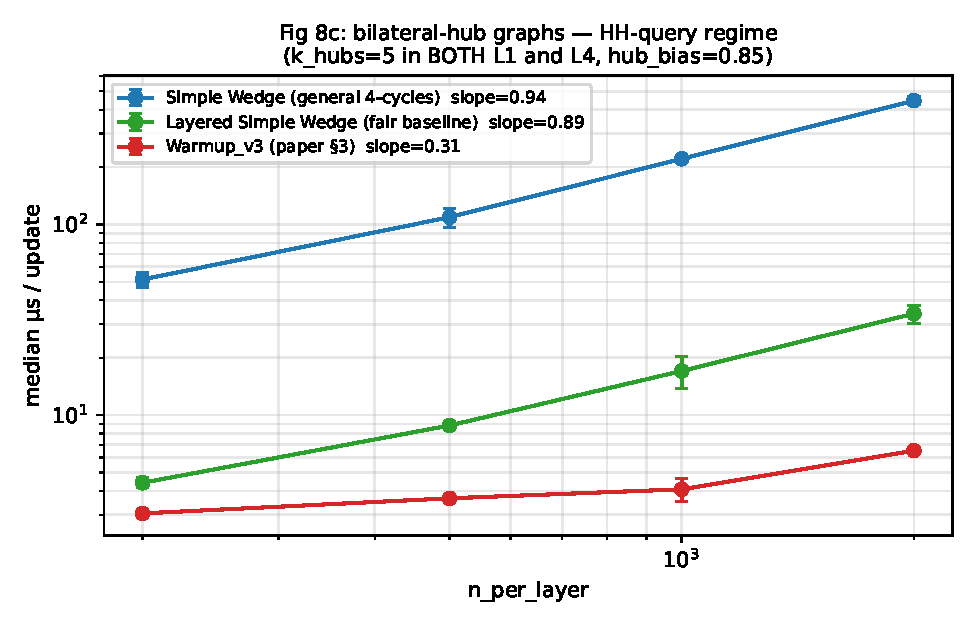
\includegraphics[width=\linewidth]{figures/fig8c_bilateral.pdf}
    \end{column}
    \begin{column}{0.45\textwidth}
      \alert{The machinery pays off where there are bilateral hubs} on both sides of the cyclic ordering.

      \vspace{0.5em}
      On simpler inputs (unilateral hubs, sparse, no hubs):
      \begin{itemize}
        \item the \emph{wedge baseline already captures most of the benefit};
        \item the class-routing layer is overhead.
      \end{itemize}

      \vspace{0.5em}
      So the routing machinery is not a generic accelerant -- it locates a \alert{specific structural regime} where FMM bandwidth pays for itself.
    \end{column}
  \end{columns}
\end{frame}

% ---------------------------------------------------------------
\begin{frame}{Takeaway}
  Two angles converged at the same pressure point:
  \begin{itemize}
    \item \alert{Algebraic} (Lemma): one constraint binds, and it is the FMM one.
    \item \alert{Empirical}: one input regime fires, and it is the bilateral-hub one.
  \end{itemize}

  \vspace{0.5em}
  Both say: the surrounding machinery exists \alert{to feed one well-conditioned FMM step}.

  \vspace{0.8em}
  \textbf{Open directions:}
  \begin{itemize}
    \item Push the closed-form bound to the real $\omega \approx 2.371$.
    \item Other cyclic-join sizes: 5-cycles, 6-cycles, $k$-cycles.
    \item Adaptive routing: detect bilateral-hub regimes online, fall back otherwise.
  \end{itemize}

  \vspace{0.5em}
  More broadly: \alert{IVM for cyclic joins} is a clean lens on the FMM-vs-streaming tension.
\end{frame}

% ---------------------------------------------------------------
\begin{frame}[standout]
  Thank you. \\[0.5em]
  \large Questions?
\end{frame}

\end{document}
